\section{Проектирование интеллектуальной справочной системы по библиографии}
\label{sec:designing}

\subsection{Интеллектуальная справочная система по библиографии}

В настоящее время существует реализация базы знаний по библиографии, которая была разработана с использованием принципов технологии OSTIS и использует SC-код как средство представления знаний, который является формальным языком описания знаний, который позволяет представлять информацию в виде семантической сети (рис. \ref{fig:bib-start-page}).\cite{OSTISBibliography}

\begin{figure}[H]
    \centering
    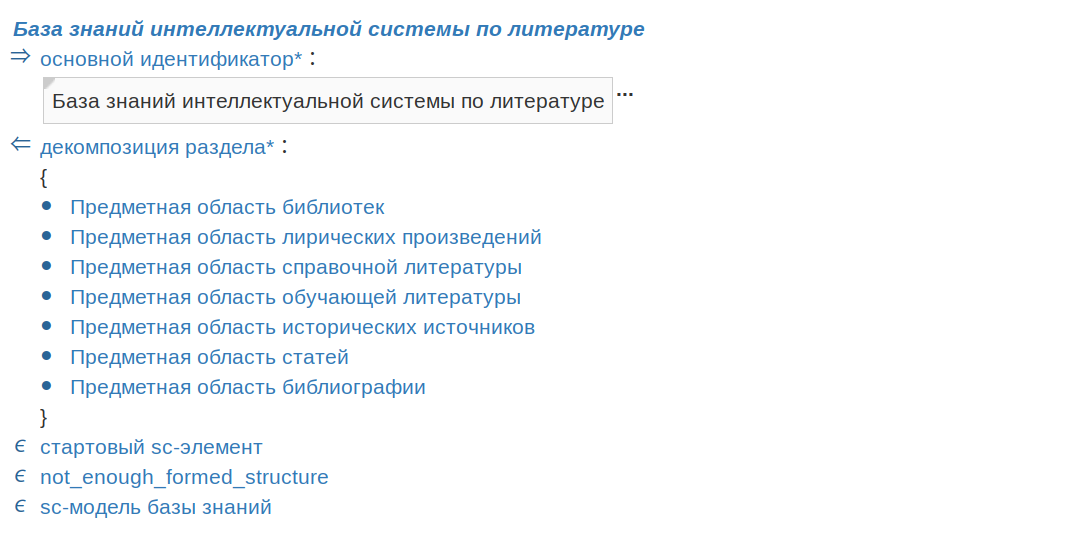
\includegraphics[scale=0.59]{imgs/bib-start-page.png}
    \caption{Стартовая страница интеллектуальной справочной системы по библиографии}
    \label{fig:bib-start-page}
\end{figure}

В данной базе знаний уже сформирована сложная иерархия предметных областей, включающая в себя различные формы литературы, в том числе лирические произведения, справочная литература, обучающая литература, исторические источники, статьи, художественная литература. Также в иерархию предметных областей входит предметная область библиотек, как неотъемлемая часть библиографии. (рис. \ref{fig:bib-structure})
\begin{figure}[H]
    \centering
    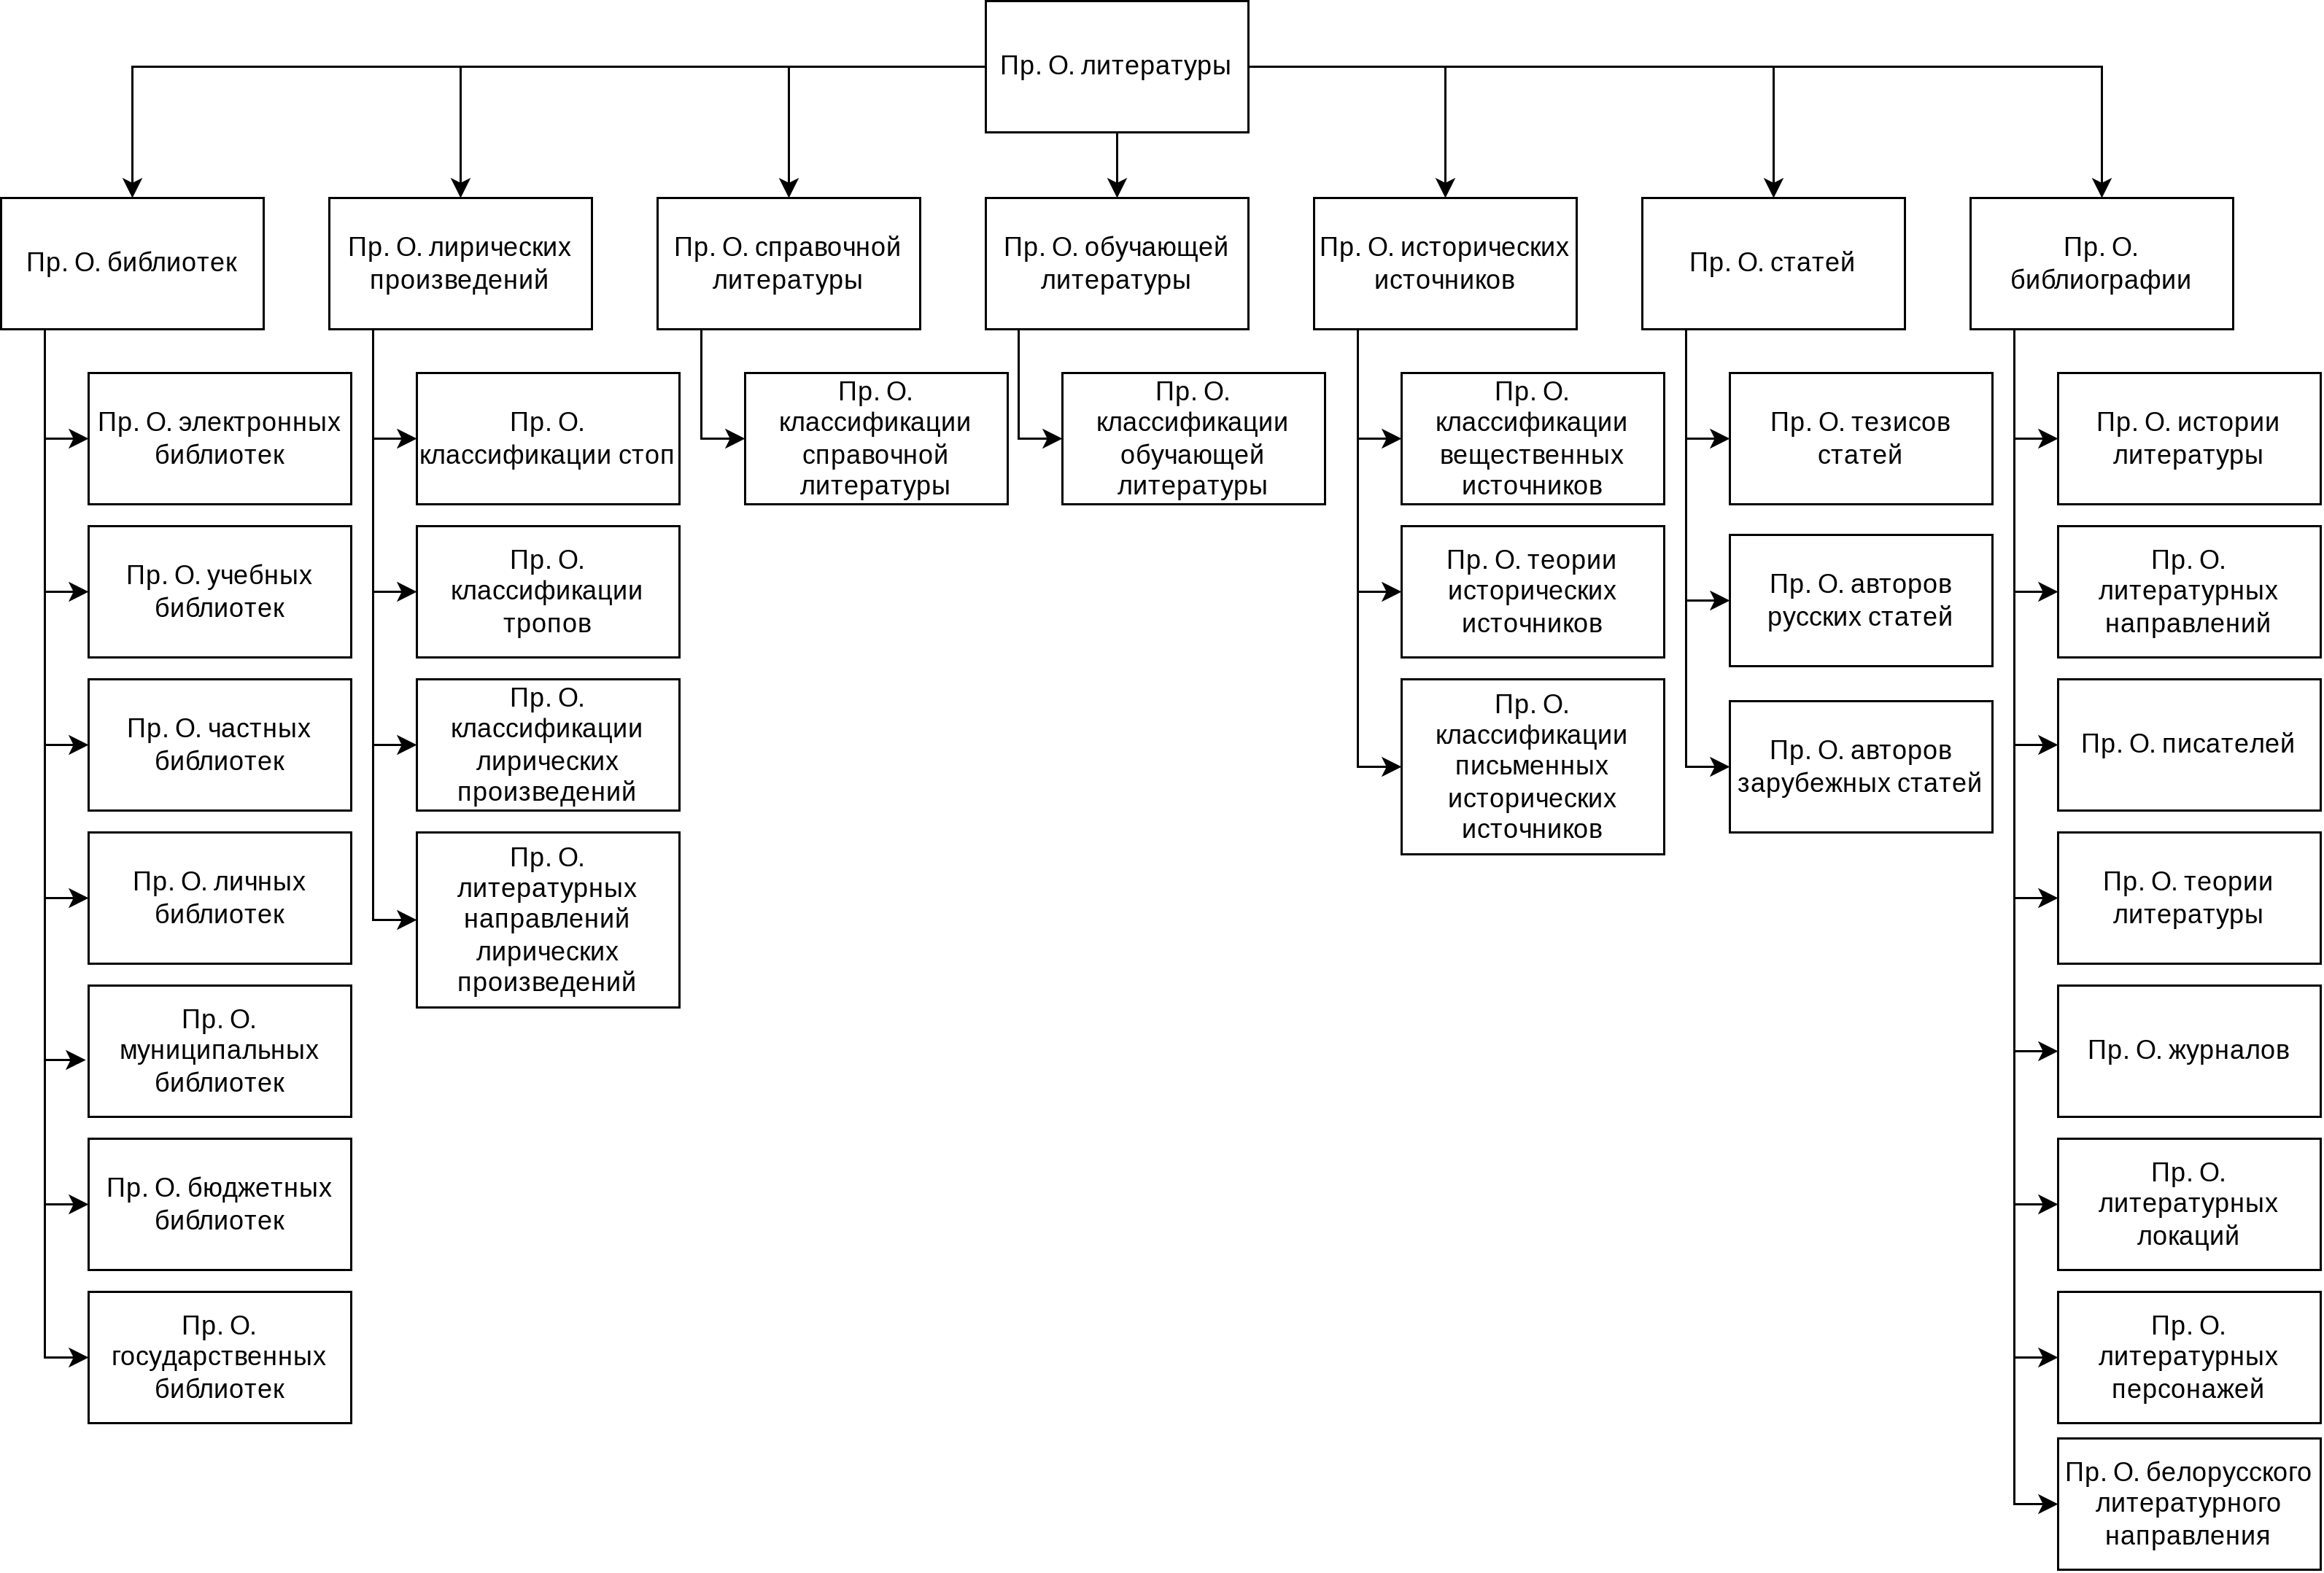
\includegraphics[scale=0.14]{imgs/existing_diag.drawio.png}
    \caption{Иерархия предметных областей базы знаний интеллектуальной справочной системы по библиографии}
    \label{fig:bib-structure}
\end{figure}

\subsection{Предметная область ранобе и её частные предметные области}

Отличительными особенностями ранобе, как направления литературы является:
\begin{itemize}
    \item Обязательное наличие иллюстраций, которые часто стилизованы под японскую анимацию. Иллюстрации в ранобе играют важную роль, так как они помогают читателю представить себе персонажей и события, происходящие в книге.

    \item В ранобе часто используются популярные концепции, такие как <<Король демонов>> и <<девочка-волшебница>>, которые являются ключевыми элементами сюжета и помогают создать уникальную атмосферу. Эти концепции могут быть использованы в разных жанрах ранобе, от приключенческих и фэнтезийных до романтических и научно-фантастических.

    \item Для этого направления литературы используются специфические жанры, такие как сёнэн (манга и аниме для мальчиков), сейнен (манга и аниме для взрослых мужчин), сёдзе (манга и аниме для девочек), хентай (эротическая манга и аниме) и другие. Эти жанры помогают читателю быстрее определить, какой тип ранобе он читает, и что он может ожидать от сюжета и персонажей.
\end{itemize}

Для описания этих уникальных особенностей ранобе в базу знаний интеллектуальной справочной системы по библиографии будут добавлены соответствующие предметные области и построения наиболее полной предметной области ранобе, было решено дополнить уже существующую иерархию предметных областей предметными областями японского литературного направления, ранобе, авторов ранобе, иллюстраторов ранобе, концепций, распространенных в ранобе, а также жанров ранобе. (рис. \ref{fig:new_structure})
\begin{figure}[H]
    \centering
    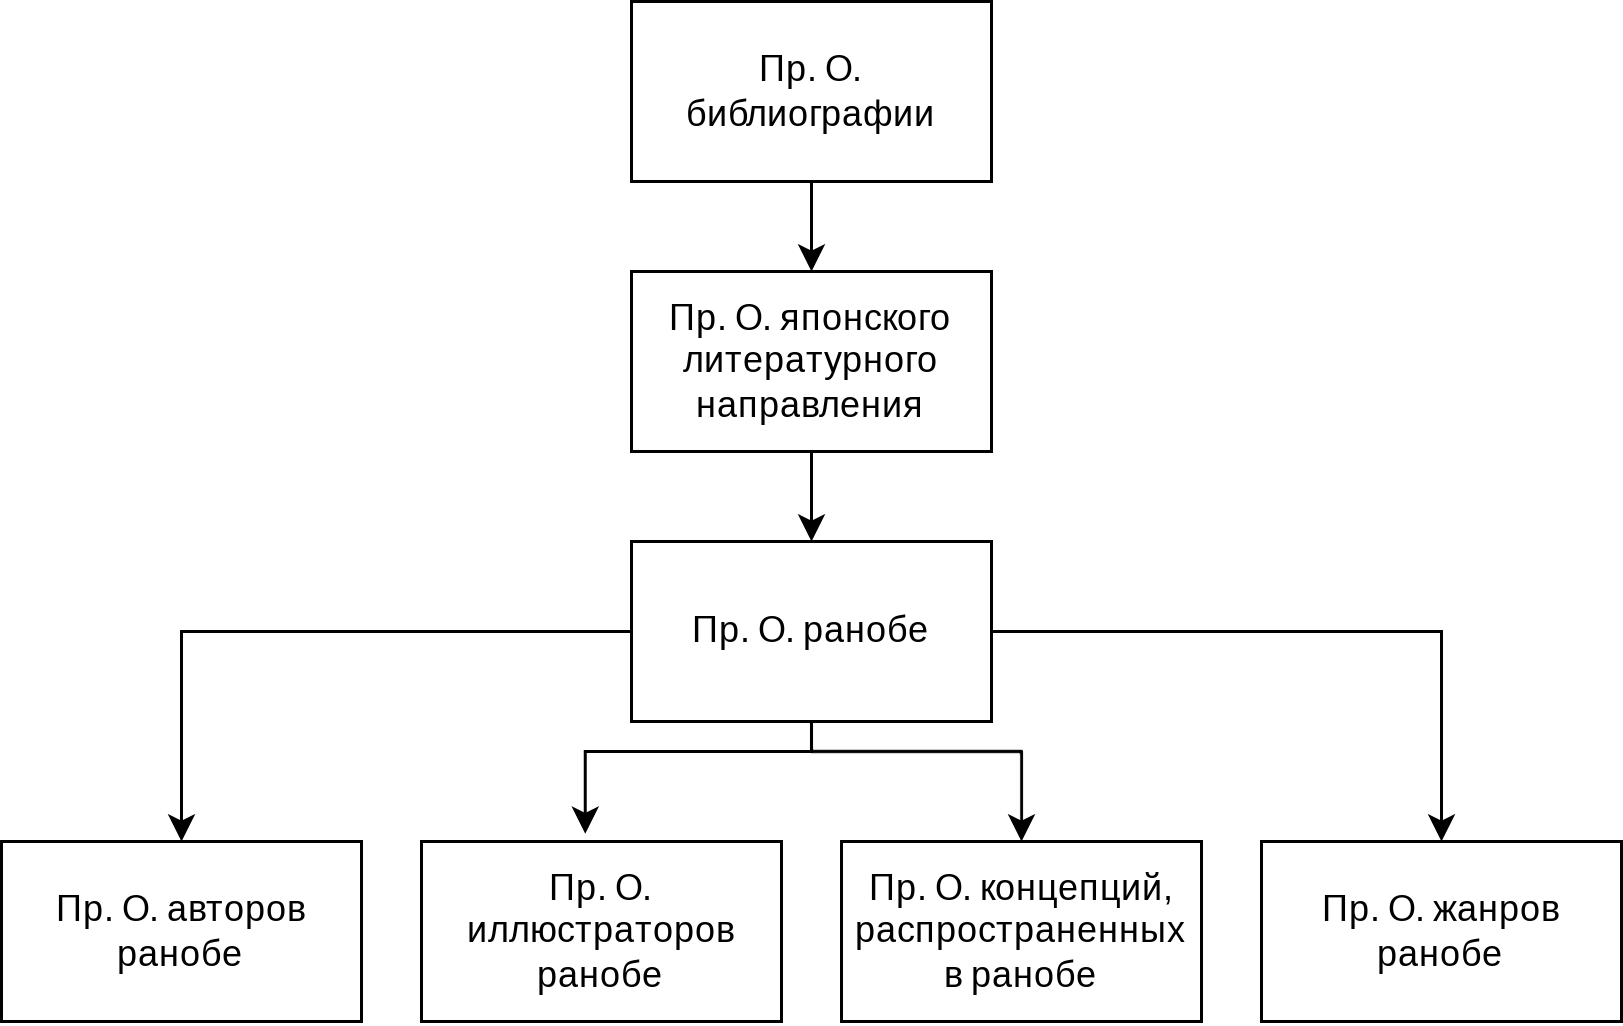
\includegraphics[scale=0.2]{imgs/new.drawio.png}
    \caption{Иерархия предметных частных предметных областей предметной области ранобе}
    \label{fig:new_structure}
\end{figure}

\subsection{Описание пользователя интеллектуальной справочной системы по библиографии}

Интеллектуальная справочная система может быть полезна различным типам пользователей, включая исследователей, ученых, переводчиков и читателей ранобе. Для каждого типа пользователя предусмотрены соответствующие сценарии использования, которые позволяют им максимально эффективно использовать систему в своих целях.

Исследователи и ученые могут использовать интеллектуальную справочную систему для поиска информации о конкретных темах, связанных с ранобе или другими литературными произведениями. Они могут использовать систему для поиска определенных авторов или персонажей, изучения специфических жанров или анализа тенденций в литературе.

Переводчики могут использовать интеллектуальную справочную систему для получения информации о персонажах, терминах и жаргоне, используемых в ранобе. Они также могут использовать систему для изучения специфических культурных и исторических аспектов, связанных с переводом ранобе на другие языки.

Читатели ранобе могут использовать интеллектуальную справочную систему для поиска информации о конкретных ранобе, включая описание персонажей, их отношения, место и время действия, а также информацию об авторе, иллюстраторе, годе выпуска и других деталях. Они могут также использовать систему для изучения истории и культуры, связанных с конкретным ранобе, или для поиска советов по чтению и рекомендаций. (рис. \ref{fig:usecases})

\begin{figure}[H]
    \centering
    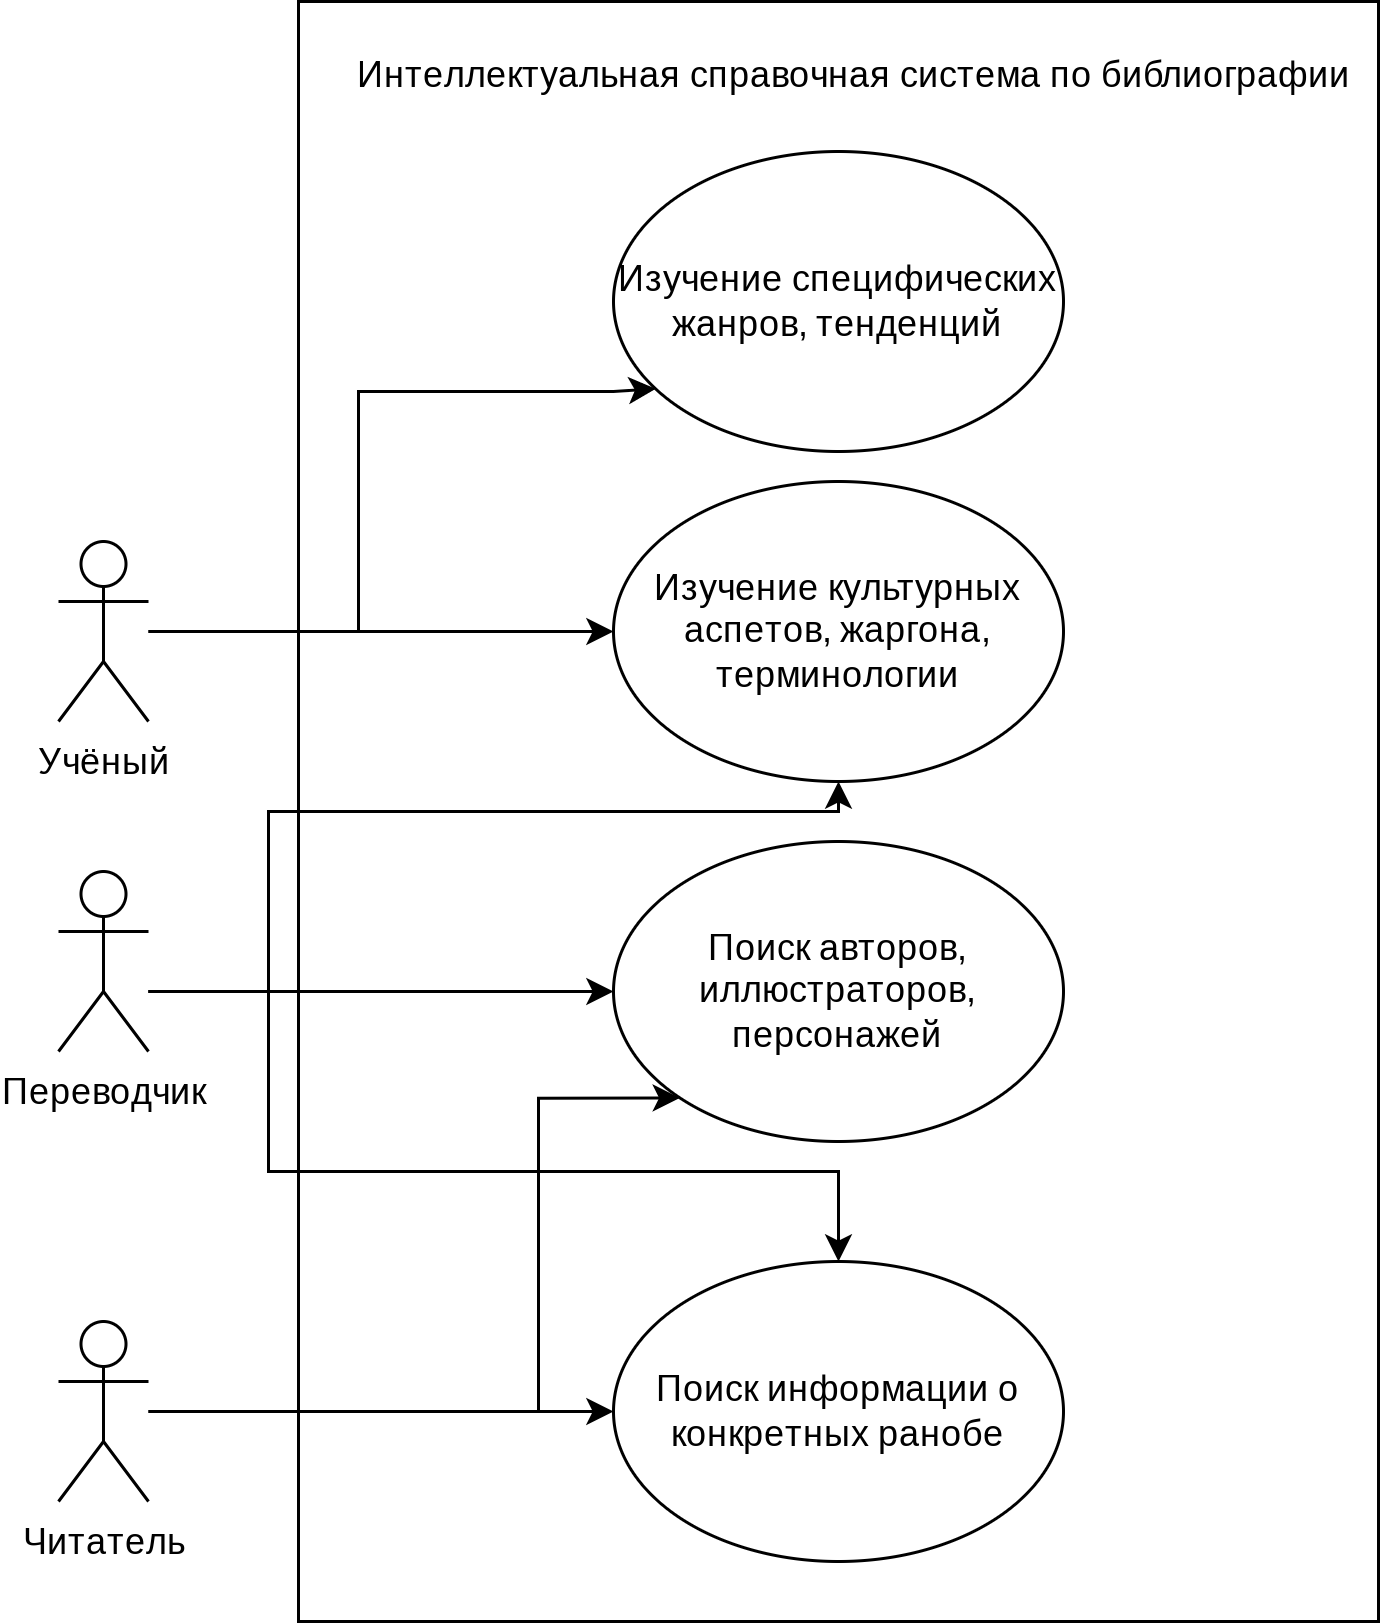
\includegraphics[scale=0.2]{imgs/usecases.drawio.png}
    \caption{Сценарии использования интеллектуальной справочной системы по библиографии пользователем}
    \label{fig:usecases}
\end{figure}

\subsection{Спецификация предметной области ранобе}

При формализации предметной области необходимо учитывать множество факторов, таких как ее цели, задачи, объекты и субъекты исследования. Определение родительской предметной области является важным шагом в этом процессе, поскольку это позволяет определить ее место в иерархической структуре знаний и установить связь с другими предметными областями. Предметная область ранобе является дочерней предметной областью для предметной области японского литературного направления.

Определение максимальных и немаксимальных классов исследования позволяет определить, какие аспекты предметной области будут рассмотрены в рамках исследования, а также определить возможные направления развития данной области знаний. Для предметной области ранобе максимальным классом исследования будет ранобе-индустрия, что включает всех людей, процессы, объекты и явления связанные с ранобе, немаксимальными же классами являются понятия <<ранобе>>, <<писатель>> и т.д.

Важным аспектом формализации предметной области является также определение исследуемых отношений, для предметной области ранобе такими отношениями будут <<автор*>>, <<иллюстратор*>>, <<характер*>>, <<конфликт*>>, <<персонажи произведения*>>, <<язык оригинала*>>.

В случае неатомарных предметных областей, определение списка дочерних предметных областей является необходимым шагом для более детального исследования каждой из этих областей. Это также помогает определить более точную иерархическую структуру знаний и установить связи между различными предметными областями.

Таким образом, спецификация предметной области ранобе:

\begin{SCn}
    \scnheader{Предметная область ранобе}
    \scntext{системный идентификатор}{subject\_domain\_of\_ranobe}
    \begin{scnrelfromlist}{основной идентификатор}
        \scnfileitem{Предмемтная область ранобе}
        \begin{scnindent}
            \scniselement{русский язык}
        \end{scnindent}
        \scnfileitem{Subject domain of ranobe}
        \begin{scnindent}
            \scniselement{английский язык}
        \end{scnindent}
    \end{scnrelfromlist}

    \scnrelto{частная предметная область}{Предметная область японского литературного направления}
    \begin{scnrelfromlist}{частная предметная область}
        \scnitem{Предметная область авторов ранобе}
        \scnitem{Предметная область иллюстраторов ранобе}
        \scnitem{Предметная область концепций, распространенных в ранобе}
        \scnitem{Предметная область жанров ранобе}
    \end{scnrelfromlist}
    \scnhaselementrole{максимальный класс объектов исследования}{ранобе-индустрия}
    \begin{scnhaselementrolelist}{немаксимальный класс объектов исследования}
        \scnitem{ранобе}
        \scnitem{писатель}
    \end{scnhaselementrolelist}

    \begin{scnhaselementrolelist}{исследумое отношение}
        \scnitem{автор*}
        \scnitem{иллюстратор*}
        \scnitem{характер*}
        \scnitem{конфликт*}
        \scnitem{персонажи произведения*}
        \scnitem{язык оригинала*}
    \end{scnhaselementrolelist}

    \scniselement{предметная область}
\end{SCn}

\subsection{Конкретные сущности в базе знаний}

Для того, чтобы система могла успешно выполнять свои прямые обязанности, в базе знаний должны быть формализованы конкретные сущности, а именно сами ранобе. Каждое ранобе должно содержать множество информации, необходимой для предоставления максимально подробной и полезной информации пользователю.

Среди формализованных знаний должны быть указаны автор и иллюстратор ранобе. Это важно для того, чтобы пользователь мог найти другие произведения автора или иллюстратора, которые могут быть ему интересны. Также важно знать язык оригинала, поскольку это позволяет определить, на каком языке нужно искать переводы ранобе. (см. приложение А).

Для того, чтобы предоставить полную информацию, необходимо указать персонажей - их пол, расу и т.д. Описание на естественном языке также должно быть доступно, чтобы пользователь мог получить представление о том, о чем идет речь. Иллюстрации могут помочь визуализировать персонажей и события. Пример формализации персонажа приведён ниже:

\begin{SCn}
    \scnheader{Киётака Аянокоджи}
    \scntext{системный идентификатор}{char\_Kiyotaka\_Ayanokouji}
    \begin{scnrelfromlist}{основной идентификатор}
        \scnfileitem{Киётака Аянокоджи}
        \begin{scnindent}
            \scniselement{русский язык}
        \end{scnindent}
        \scnfileitem{Kiyotaka Ayanokouji}
        \begin{scnindent}
            \scniselement{английский язык}
        \end{scnindent}
    \end{scnrelfromlist}
    \begin{scniselementrolelist}{ключевой sc-элемент}
        \scnitem{Изображение персонажа (Киётака Аянокоджи)}
        \scnitem{Описание персонажа (Киётака Аянокоджи)}
    \end{scniselementrolelist}
    \scniselementrole{главный герой}{...}
    \begin{scnindent}
        \scnrelfrom{персонажи произведения}{<<Класс превосходства>>}
    \end{scnindent}
    \scniselement{человек}
    \scniselement{мужчина}
\end{SCn}

%\begin{listing}[H]
%    \begin{verbatim}
%char_Kiyotaka_Ayanokouji
%=> nrel_main_idtf: [Киётака Аянокоджи] (* <-lang_ru;; *);
%<- person; <- male;
%<- rrel_key_sc_element: ... (*
%        => nrel_main_idtf:
%            [Изображение персонажа(Киётака Аянокоджи)]
%            (* <- lang_ru;; *);;
%        <= nrel_sc_text_translation:
%            ...
%            (* -> "file://images/char_Kiyotaka_Ayanokouji.jpg"
%                (* => nrel_format: format_jpg;; *);;
%            *);;
%    *);
%    ... (*
%        => nrel_main_idtf: [Описание персонажа(Киётака Аянокоджи)]
%            (* <-lang_ru;; *);;
%        <= nrel_sc_text_translation: 
%            ...
%            (*
%                -> "file://content/char_Kiyotaka_Ayanokouji.html"
%                    (* <-lang_ru;;
%                        => nrel_format: format_html;; *);;
%            *);;
%    *);;
%    \end{verbatim}
%
%    \caption{Пример формализации персонажа в базе знаний интеллектуальной справочной системы по библиографии}
%    \label{lst:character_example}
%\end{listing}

Для полного охвата информации о ранобе необходимо указать жанр произведения, год выпуска и обложки. Жанры ранобе могут быть специфическими, такими как сёнэн или сёдзе, и должны быть указаны отдельно. Год выпуска также важен для определения того, насколько новое произведение, и соответственно, какая информация может быть актуальной. Обложки книг также являются важным элементом, поскольку они могут помочь пользователю найти нужное произведение в магазине или в библиотеке. Для описания каких-либо свойств произведения необходимо использовать относительные понятия (отношения), пример формализации онтосительного понятия:

\begin{SCn}
    \scnheader{иллюстратор}
    \scntext{системный идентификатор}{nrel\_illustrator}
    \begin{scnrelfromlist}{основной идентификатор}
        \scnfileitem{иллюстратор*}
        \begin{scnindent}
            \scniselement{русский язык}
        \end{scnindent}
        \scnfileitem{illustrator*}
        \begin{scnindent}
            \scniselement{английский язык}
        \end{scnindent}
    \end{scnrelfromlist}
    
    \scnrelfrom{первый домен}{человек}
    \scnrelfrom{второй домен}{литературное произведение}

    \scniselement{бинарное отношение}
    \scniselement{ориентированное отношение}
    \scniselement{асимметричное отношение}
    \scniselement{антитранзитивное отношение}

    \scniselementrole{ключевой sc-элемент}{Определение (иллюстратор*)}
\end{SCn}



В базе знаний могут присутствовать ссылки на дополнительные материалы, такие как интервью с автором, видеообзоры, рецензии и т.д. Это может помочь пользователям получить более полное представление о произведении и его создателе. Кроме того, важно учесть, что ранобе могут иметь адаптации в других форматах, например, манга или аниме. В базе знаний также могут присутствовать сведения об этих адаптациях, чтобы пользователь мог узнать больше о мире ранобе и его персонажах.

В итоге, чем больше информации содержится в базе знаний о ранобе, тем более полезным и эффективным становится интеллектуальная справочная система для пользователей.

\subsection{Вывод}
На этапе проектирования была проведена работа по изучению иерархии предметных областей в рамках базы знаний по библиографии, с целью определения наиболее релевантных и информативных областей для добавления знаний о ранобе. Были также определены дополнительные требования к разрабатываемым предметным областям, с учетом особенностей ранобе, таких как жанры, авторы, персонажи и т.д.

Особое внимание уделено формализации конкретных ранобе. Для обеспечения максимальной полезности и удобства использования системы, для каждого ранобе должны быть формализованы все необходимые данные, включая автора и иллюстратора ранобе, язык оригинала, персонажей произведения, жанры, год выпуска, обложки и другие характеристики. Более того, также должны быть представлены иллюстрации из ранобе, манги или аниме, а также описания на естественном языке.

Все вышеперечисленные меры направлены на обеспечение максимальной эффективности и полезности интеллектуальной справочной системы по библиографии, включая добавление знаний о ранобе. Они позволят пользователям получать максимально подробную и полезную информацию о ранобе, а также более эффективно использовать систему для своих нужд.
